\clearpage
\section{Digression on Caches}

This experimental section is distinguished into 2 parts. First we show a
few different opportunities to access a linked list, and an array,
respectively. Allows keeping our purpose in mind, we want to illustrate
the cache hierarchy. Secondly, we go into details and clarify a raising
question. Which finally leads to the answer we are looking for.

All experiments were executed on a MacBook Pro with a Intel(R) Core(TM)
i5-3230M CPU @ 2.60GHz and 3 cache levels (L1d=32KB, L1i=32KB, L2=256KB,
and L3=3MB). During the experiments there were other processes running
on the MacBook, this is why these results should be seen as proof of
concept.

\subsection{Configuration}\label{configuration-3}

The configuration is for all experiments identical.

\begin{longtable}[c]{@{}cccc@{}}
\toprule
Reps & Operations & Working Set Sizes & Addresses\tabularnewline
\midrule
\endhead
3 & 234 & 210 - 228 & 228\tabularnewline
\bottomrule
\end{longtable}

We are aware that the number of repetitions is very small, but we
consider these experiments as a \emph{proof of concept}. So 3
repetitions should be good enough.

There are parameters listed within the configuration files which are
\textbf{not} used for this experiments! These are only listed to keep
the experimental framework working.

\begin{itemize}
\tightlist
\item
  Fragmentation factor
\item
  Store ratio
\end{itemize}

As explained above we generate for each working set size a standalone
\texttt{C} file. which is complied with \texttt{gcc} in version 4.8.5
with following compiler flags \texttt{-std=c99} and \texttt{-O0}.

\hypertarget{access-opportunities}{\subsection{Access
opportunities}\label{access-opportunities}}

\hypertarget{linked-list}{\paragraph{Linked List}\label{linked-list}}

This section presents code snippets and performance results of accessing
a linked list to illustrate the cache hierarchy.

\hypertarget{sequential-access-with-2-loops}{\subparagraph{Sequential
access with 2 loops}\label{sequential-access-with-2-loops}}

The code snippet below shows how to access the linked list in a
sequential manner. All list elements are sequentially linked
corresponding to there position in (contiguous) memory. This approach
uses two nested loops.

\begin{Shaded}
\begin{Highlighting}[]
\DataTypeTok{static} \DataTypeTok{uint64_t} \NormalTok{access_read() \{}
  \KeywordTok{struct} \NormalTok{l * cur = &list[}\DecValTok{0}\NormalTok{];}
  \DataTypeTok{uint64_t} \NormalTok{start = getTimeMicrosecs();}
  \KeywordTok{for}\NormalTok{(}\DataTypeTok{int} \NormalTok{i = }\DecValTok{0}\NormalTok{; i < ITERS; i++)}
  \NormalTok{\{}
    \KeywordTok{for}\NormalTok{(}\DataTypeTok{int} \NormalTok{e = }\DecValTok{0}\NormalTok{; e < ELEMS; e++)}
    \NormalTok{\{}
      \NormalTok{cur = cur->n;}
      \NormalTok{(}\DataTypeTok{void}\NormalTok{)cur->pad[}\DecValTok{0}\NormalTok{];}
    \NormalTok{\}}
  \NormalTok{\}}
  \KeywordTok{return} \NormalTok{getTimeMicrosecs() - start;}
\NormalTok{\}}
\end{Highlighting}
\end{Shaded}

\Cref{ll-seqread-nl} presents the performance of the code above. As expected
the cache hierarchy is observable. However, performance is not that
good. How poor it really is illustrates the next experiment.

\begin{figure}[htbp]
\centering
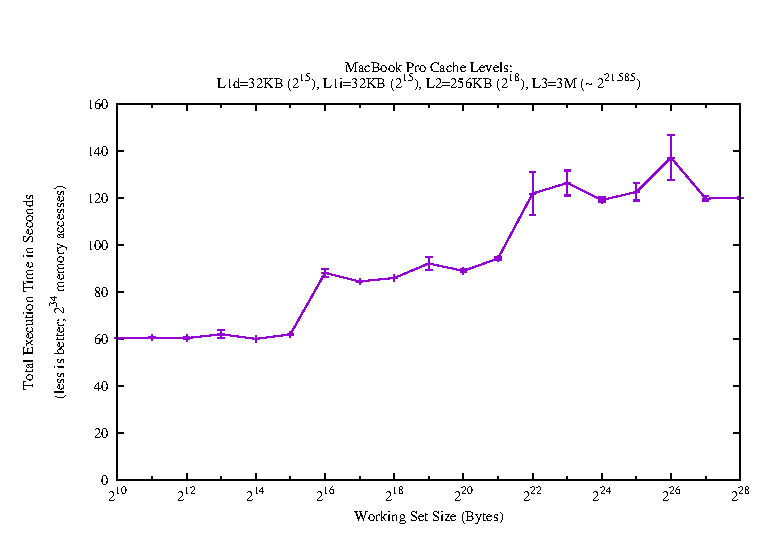
\includegraphics{appendix/plots-cache-measurements/plot-linked-list-2-loops}
\caption{Linked List, Sequential Read, and Nested Loop}
\label{ll-seqread-nl}
\end{figure}

\hypertarget{sequential-access-with-single-loop}{\subparagraph{Sequential
access with single loop}\label{sequential-access-with-single-loop}}

This approach is similar to the one above, but instead of two nested
loops a single loop is used. All list elements are sequentially linked
corresponding to there position in (contiguous) memory.

\begin{Shaded}
\begin{Highlighting}[]
\DataTypeTok{static} \DataTypeTok{uint64_t} \NormalTok{access_read() \{}
  \KeywordTok{struct} \NormalTok{l * cur = &list[}\DecValTok{0}\NormalTok{];}
  \DataTypeTok{uint64_t} \NormalTok{start = getTimeMicrosecs();}
  \KeywordTok{for}\NormalTok{(}\DataTypeTok{int} \NormalTok{i = }\DecValTok{0}\NormalTok{; i < ITERS * ELEMS; i++)}
  \NormalTok{\{}
    \NormalTok{cur = cur->n;}
    \NormalTok{(}\DataTypeTok{void}\NormalTok{)cur->pad[}\DecValTok{0}\NormalTok{];}
  \NormalTok{\}}
  \KeywordTok{return} \NormalTok{getTimeMicrosecs() - start;}
\NormalTok{\}}
\end{Highlighting}
\end{Shaded}

\Cref{app:ll-seqread-sl} illustrates the performance of the code from above. As
expected the results shows the typical shape. Remember the experiment
was not the only job running, this is why the shape not totally sharp.
This figure is used as baseline for the following experiments.

\begin{figure}[htbp]
\centering
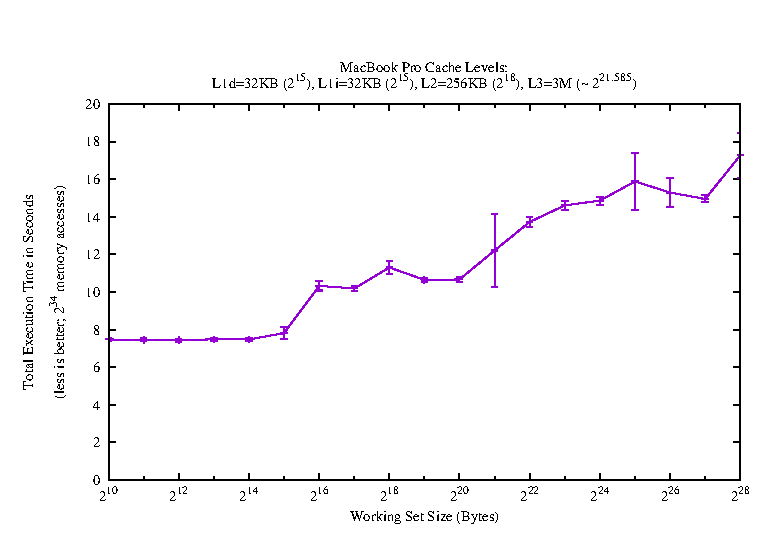
\includegraphics{appendix/plots-cache-measurements/plot-linked-list}
\caption{Linked List, Sequential Read, and Single Loop}
\label{app:ll-seqread-sl}
\end{figure}

\hypertarget{array}{\paragraph{Array}\label{array}}

This section presents different ways to compute the index of the array.
The aim is illustrate the influence of computing the index of the
current element on the actual measurements.

\hypertarget{sequential-access-with-2-loops-1}{\subparagraph{Sequential
access with 2 loops}\label{sequential-access-with-2-loops-1}}

The code snippet below shows how the array is accessed. This approach
uses to nested loop. The outer-one determines the number accesses on a
single element with the array. The inner-one ensures that keep walking
through the array.

\begin{Shaded}
\begin{Highlighting}[]
\DataTypeTok{static} \DataTypeTok{uint64_t} \NormalTok{access_read() \{}
  \DataTypeTok{uint64_t} \NormalTok{start = getTimeMicrosecs();}
  \KeywordTok{for}\NormalTok{(}\DataTypeTok{int} \NormalTok{i = }\DecValTok{0}\NormalTok{; i < ITERS; i++)}
    \KeywordTok{for}\NormalTok{(}\DataTypeTok{int} \NormalTok{j = }\DecValTok{0}\NormalTok{; j < ELEMS; j++)}
      \NormalTok{(}\DataTypeTok{void}\NormalTok{)list[j].pad[}\DecValTok{0}\NormalTok{];}
  \KeywordTok{return} \NormalTok{getTimeMicrosecs() - start;}
\NormalTok{\}}
\end{Highlighting}
\end{Shaded}

\Cref{app:arr-seqread-nl} presents the performance of the code above. Obviously
the cache hierarchy is not observable. Instead the performance seams to
be independent of the working set size. We continue with a few more
experiments on array before taking a closer look at this effect.

\begin{figure}[htbp]
\centering
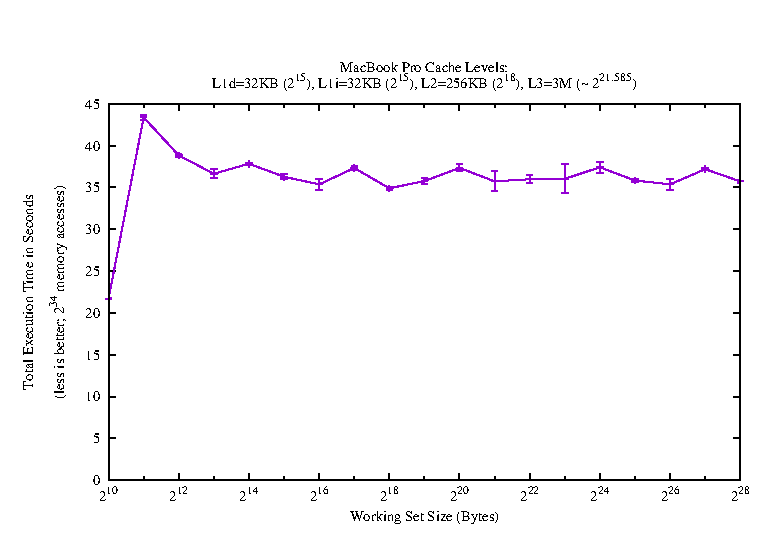
\includegraphics{appendix/plots-cache-measurements/plot-array-2-loops}
\caption{Array, Sequential Read, and Nested Loop}
\label{app:arr-seqread-nl}
\end{figure}

\hypertarget{sequential-access-with-single-loop-and-modulo}{\subparagraph{Sequential
access with single loop and
modulo}\label{sequential-access-with-single-loop-and-modulo}}

The code snippet below illustrates an approach which uses only one loop.
This requires a modulo operation to ensure to stay within the array
bounds.

\begin{Shaded}
\begin{Highlighting}[]
\DataTypeTok{static} \DataTypeTok{uint64_t} \NormalTok{access_read() \{}
  \DataTypeTok{uint64_t} \NormalTok{start = getTimeMicrosecs();}
  \KeywordTok{for}\NormalTok{(}\DataTypeTok{int} \NormalTok{i = }\DecValTok{0}\NormalTok{; i < ITERS * ELEMS; i++)}
    \NormalTok{(}\DataTypeTok{void}\NormalTok{)list[i%ELEMS].pad[}\DecValTok{0}\NormalTok{];}
  \KeywordTok{return} \NormalTok{getTimeMicrosecs() - start;}
\NormalTok{\}}
\end{Highlighting}
\end{Shaded}

\Cref{app:arr-seqread-sl} shows the performance of the code above. Again the
performance seams to be independent of the working set size. However,
there is a significant performance improvement compared to the approach
with two loops.

\begin{figure}[htbp]
\centering
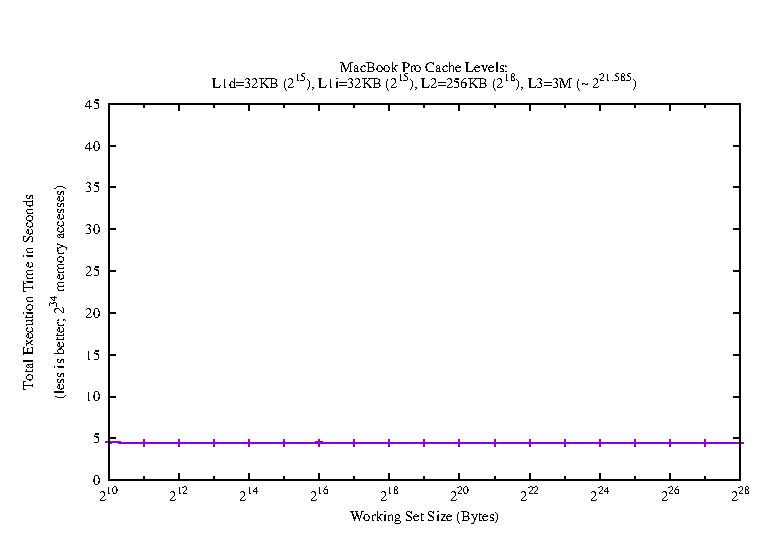
\includegraphics{appendix/plots-cache-measurements/plot-array-modulo-seq}
\caption{Array, Sequential Read, and Single Loop}
\label{app:arr-seqread-sl}
\end{figure}

\hypertarget{sequential-access-with-single-loop-and-modulo-linked-list-style}{\subparagraph{Sequential
access with single loop and modulo (linked list
style)}\label{sequential-access-with-single-loop-and-modulo-linked-list-style}}

The code snipped below presents an approach which used only one loop,
which requires a modulo operation to care about the array bounds.
Further, the coding style is like used a linked lists. There is an
additional variable \texttt{cur} which holds the address of the element
to access. The reason for this experiment that all experiments with
arrays so far do not show the cache hierarchy. To become as comparable
as possible we use this linked list like syntax.

\begin{Shaded}
\begin{Highlighting}[]
\DataTypeTok{static} \DataTypeTok{uint64_t} \NormalTok{access_read() \{}
  \KeywordTok{struct} \NormalTok{l * cur = &list[}\DecValTok{0}\NormalTok{];}
  \DataTypeTok{uint64_t} \NormalTok{start = getTimeMicrosecs();}
  \KeywordTok{for}\NormalTok{(}\DataTypeTok{int} \NormalTok{i = }\DecValTok{0}\NormalTok{; i < ITERS * ELEMS; i++)\{}
    \NormalTok{cur = &list[i%ELEMS];}
    \NormalTok{(}\DataTypeTok{void}\NormalTok{)cur->pad[}\DecValTok{0}\NormalTok{];}
  \NormalTok{\}}
  \KeywordTok{return} \NormalTok{getTimeMicrosecs() - start;}
\NormalTok{\}}
\end{Highlighting}
\end{Shaded}

\Cref{app:array-seqread-sl} below shows the performance of the code above. Again the
performance seams to be independent of the working set size. However,
the performance is slightly worse than the performance of the previous
experiment. The explanation is as simple as: It is requires to store the
address within \texttt{cur}, the approach from above computes address
and stores it in a register.

\begin{figure}[htbp]
\centering
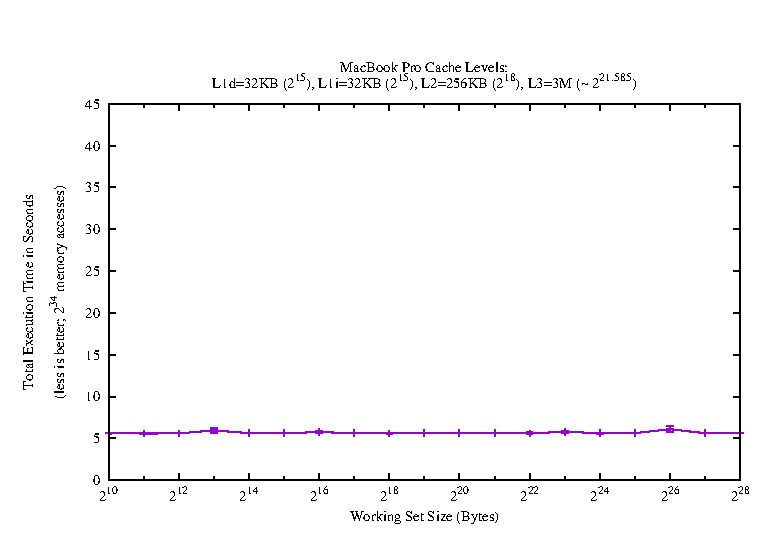
\includegraphics{appendix/plots-cache-measurements/plot-array-modulo-seq-2}
\caption{Array, Sequential Read, and Single Loop}
\label{app:array-seqread-sl}
\end{figure}

\hypertarget{sequential-access-with-single-loop-and-modulo-read-whole-payload}{\subparagraph{Sequential
access with single loop and modulo (read whole
payload)}\label{sequential-access-with-single-loop-and-modulo-read-whole-payload}}

The code snippet below presents an approach similar to those from above
with one difference: The whole payload is read (instead of simply
reading on element).

\begin{Shaded}
\begin{Highlighting}[]
\DataTypeTok{static} \DataTypeTok{uint64_t} \NormalTok{access_read() \{}
  \KeywordTok{struct} \NormalTok{l * cur = &list[}\DecValTok{0}\NormalTok{];}
  \DataTypeTok{uint64_t} \NormalTok{start = getTimeMicrosecs();}
  \KeywordTok{for}\NormalTok{(}\DataTypeTok{int} \NormalTok{i = }\DecValTok{0}\NormalTok{; i < ITERS * ELEMS; i++)\{}
    \NormalTok{cur = &list[i%ELEMS];}
    \KeywordTok{for}\NormalTok{(}\DataTypeTok{int} \NormalTok{j = }\DecValTok{0}\NormalTok{; j < NPAD; j++)}
      \NormalTok{(}\DataTypeTok{void}\NormalTok{)cur->pad[j];}
  \NormalTok{\}}
  \KeywordTok{return} \NormalTok{getTimeMicrosecs() - start;}
\NormalTok{\}}
\end{Highlighting}
\end{Shaded}

\Cref{app:array-seqreadall-sl} shows the result of the code from above. It was
expected to see the cache hierarchy, because we read the whole array
which is definitely larger than the cache. Nevertheless, the result is
the same as for the other array experiments. The only difference is the
worse performance yield by the additional loop.

\begin{figure}[htbp]
\centering
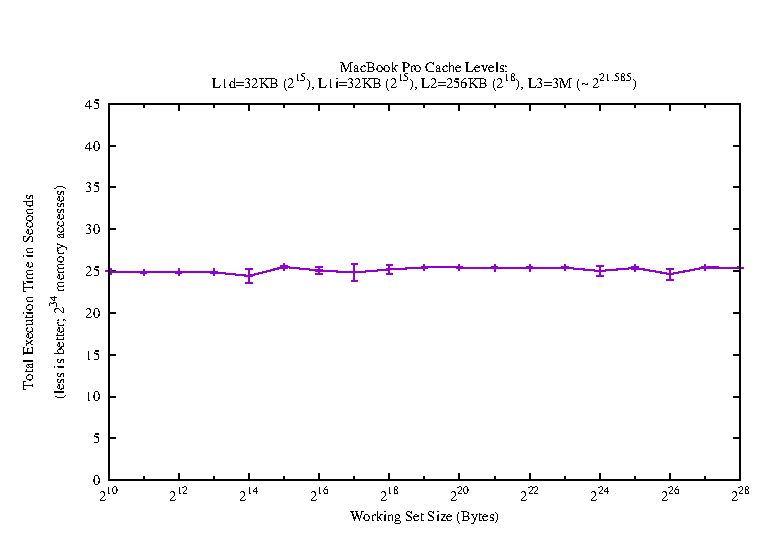
\includegraphics{appendix/plots-cache-measurements/plot-array-modulo-seq-read-all}
\caption{Array, Sequential Read All, and Single Loop}
\label{app:array-seqreadall-sl}
\end{figure}

\hypertarget{random-access-with-single-loop-and-modulo}{\subparagraph{Random
access with single loop and
modulo}\label{random-access-with-single-loop-and-modulo}}

The code snippet below presents an approach similar to those from above
with one difference: Now the array elements are access in a random
order. \texttt{mapper} contains a randomly chosen permutation of all
array indexes.

\begin{Shaded}
\begin{Highlighting}[]
\DataTypeTok{static} \DataTypeTok{uint64_t} \NormalTok{access_read() \{}
  \KeywordTok{struct} \NormalTok{l * cur = &list[}\DecValTok{0}\NormalTok{];}
  \DataTypeTok{uint64_t} \NormalTok{start = getTimeMicrosecs();}
  \KeywordTok{for}\NormalTok{(}\DataTypeTok{int} \NormalTok{i = }\DecValTok{0}\NormalTok{; i < ITERS * ELEMS; i++)\{}
    \NormalTok{cur = &list[mapper[i%ELEMS]];}
    \NormalTok{(}\DataTypeTok{void}\NormalTok{)cur->pad[}\DecValTok{0}\NormalTok{];}
  \NormalTok{\}}
  \KeywordTok{return} \NormalTok{getTimeMicrosecs() - start;}
\NormalTok{\}}
\end{Highlighting}
\end{Shaded}

The performance result is shown in \Cref{app:arr-randread-sl}. The random access order is chosen
to get rid of pre-fetching which could probably influence the execution
time. But even with random access on the array we cannot observer the
cache hierarchy. It is comparable to \emph{sequential access with single
loop and modulo (linked list style)}.

\begin{figure}[htbp]
\centering
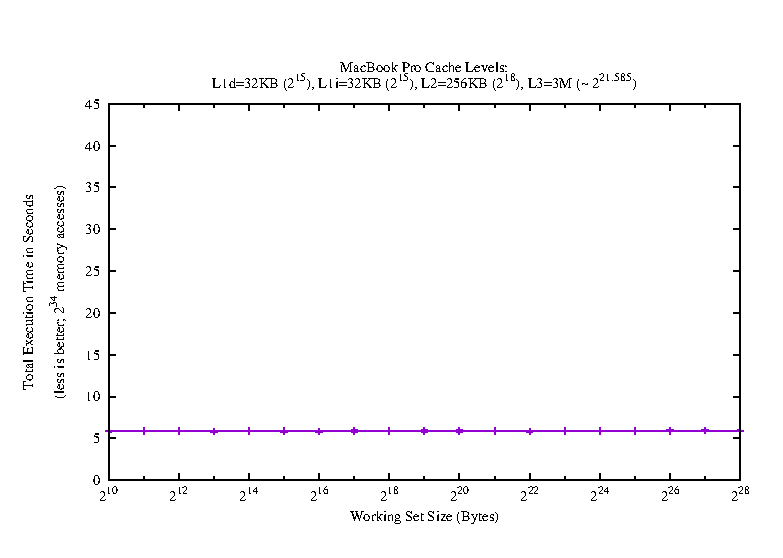
\includegraphics{appendix/plots-cache-measurements/plot-array-modulo-rand}
\caption{Array, Random Read, and Single Loop}
\label{app:arr-randread-sl}
\end{figure}

\hypertarget{summary-1}{\paragraph{Summary}\label{summary-1}}

We presented experiments on accessing two different data structures,
linked lists, and arrays, respectively. For linked lists we showed that
there is a huge performance difference in using nested loops or just a
single loop. This fact is not super surprising, but nevertheless
important to keep in mind. Also for arrays is shown that 2 nested loops
perform do not perform well. Further, we tried to measure the cache
hierarchy using just an array. Without success. Instead our experiments
show the performance differences of the different ways to access an
array. The following section will go into details why performance seams
to be independent of the working set size.

\hypertarget{the-problem}{\subsection{The problem}\label{the-problem}}

\hypertarget{definition}{\subsection{Definition}\label{definition}}

The performance curve of all experiments with array only is close to a
horizontal line, and this is unexpected behavior. It seams to be
independent of the working set size. The expected behavior would be
similar to the linked list experiments, which illustrate the cache
hierarchy.

\subsection{Analysis}\label{analysis-1}

In this section we investigate the unexpected behavior of our array
experiments from above. These experiments present constant performance
independent of the working set size.

\hypertarget{assembly-code-analysis}{\paragraph{Assembly code
analysis}\label{assembly-code-analysis}}

To simplify as much as possible we inspect only 2 code snippets from
above: - Linked list with single loop and - Array with single loop in
linked list style.

These two are the most similar one so optimal for comparison. We
disassembled the executables complied on the MacBook mentioned above.
For disassembling we are using an on-line disassembler:
\url{https://onlinedisassembler.com}.

\textbf{Linked list: C code}

\begin{Shaded}
\begin{Highlighting}[]
\DataTypeTok{static} \DataTypeTok{uint64_t} \NormalTok{access_read() \{}
  \KeywordTok{struct} \NormalTok{l * cur = &list[}\DecValTok{0}\NormalTok{];}
  \DataTypeTok{uint64_t} \NormalTok{start = getTimeMicrosecs();}
  \KeywordTok{for}\NormalTok{(}\DataTypeTok{int} \NormalTok{i = }\DecValTok{0}\NormalTok{; i < ITERS * ELEMS; i++)\{}
    \NormalTok{cur = cur->n;}
    \NormalTok{(}\DataTypeTok{void}\NormalTok{)cur->pad[}\DecValTok{0}\NormalTok{];}
  \NormalTok{\}}
  \KeywordTok{return} \NormalTok{getTimeMicrosecs() - start;}
\NormalTok{\}}
\end{Highlighting}
\end{Shaded}

\textbf{Linked list: Assembly}

\begin{verbatim}
100000ec0 <_access_read>:
100000ec0 55                     push   %rbp
100000ec1 4889e5                 mov    %rsp,         %rbp
100000ec4 4883ec20               sub    $0x20,        %rsp
100000ec8 488d0551010000         lea    0x151(%rip),  %rax # 0x100001020<_list>
100000ecf 488945f8               mov    %rax,         -0x8(%rbp)
100000ed3 e858000000             callq  0x100000f30   <_getTimeMicrosecs>
100000ed8 488945f0               mov    %rax,         -0x10(%rbp)
100000edc c745ec00000000         movl   $0x0,         -0x14(%rbp)
100000ee3 48b80000000004000000   movabs $0x400000000, %rax
100000eed 48634dec               movslq -0x14(%rbp),  %rcx
100000ef1 4839c1                 cmp    %rax,         %rcx
100000ef4 0f8319000000           jae    0x100000f13
100000efa 488b45f8               mov    -0x8(%rbp),   %rax
100000efe 488b00                 mov    (%rax),       %rax
100000f01 488945f8               mov    %rax,         -0x8(%rbp)
100000f05 8b45ec                 mov    -0x14(%rbp),  %eax
100000f08 83c001                 add    $0x1,         %eax
100000f0b 8945ec                 mov    %eax,         -0x14(%rbp)
100000f0e e9d0ffffff             jmpq   0x100000ee3
100000f13 e818000000             callq  0x100000f30   <_getTimeMicrosecs>
100000f18 482b45f0               sub    -0x10(%rbp),  %rax
100000f1c 4883c420               add    $0x20,        %rsp
100000f20 5d                     pop    %rbp
100000f21 c3                     retq   
\end{verbatim}

\textbf{Array: C code}

\begin{Shaded}
\begin{Highlighting}[]
\NormalTok{...}
\DataTypeTok{static} \DataTypeTok{uint64_t} \NormalTok{access_read() \{}
  \KeywordTok{struct} \NormalTok{l * cur = &list[}\DecValTok{0}\NormalTok{];}
  \DataTypeTok{uint64_t} \NormalTok{start = getTimeMicrosecs();}
  \KeywordTok{for}\NormalTok{(}\DataTypeTok{int} \NormalTok{i = }\DecValTok{0}\NormalTok{; i < ITERS * ELEMS; i++)\{}
    \NormalTok{cur = &list[i%ELEMS];}
    \NormalTok{(}\DataTypeTok{void}\NormalTok{)cur->pad[}\DecValTok{0}\NormalTok{];}
  \NormalTok{\}}
  \KeywordTok{return} \NormalTok{getTimeMicrosecs() - start;}
\NormalTok{\}}
\end{Highlighting}
\end{Shaded}

\textbf{Array: Assembly}

\begin{verbatim}
100000eb0 <_access_read>:
100000eb0 55                     push   %rbp
100000eb1 4889e5                 mov    %rsp,         %rbp
100000eb4 4883ec20               sub    $0x20,        %rsp
100000eb8 488d0561010000         lea    0x161(%rip),  %rax # 0x100001020<_list>
100000ebf 488945f8               mov    %rax,         -0x8(%rbp)
100000ec3 e868000000             callq  0x100000f30   <_getTimeMicrosecs>
100000ec8 488945f0               mov    %rax,         -0x10(%rbp)
100000ecc c745ec00000000         movl   $0x0,         -0x14(%rbp)
100000ed3 48b80000000004000000   movabs $0x400000000, %rax
100000edd 48634dec               movslq -0x14(%rbp),  %rcx
100000ee1 4839c1                 cmp    %rax,         %rcx
100000ee4 0f8328000000           jae    0x100000f12
100000eea 488d052f010000         lea    0x12f(%rip),  %rax # 0x100001020<_list>
100000ef1 48634dec               movslq -0x14(%rbp),  %rcx
100000ef5 4883e10f               and    $0xf,         %rcx
100000ef9 48c1e106               shl    $0x6,         %rcx
100000efd 4801c8                 add    %rcx,         %rax
100000f00 488945f8               mov    %rax,         -0x8(%rbp)
100000f04 8b45ec                 mov    -0x14(%rbp),  %eax
100000f07 83c001                 add    $0x1,         %eax
100000f0a 8945ec                 mov    %eax,         -0x14(%rbp)
100000f0d e9c1ffffff             jmpq   0x100000ed3
100000f12 e819000000             callq  0x100000f30   <_getTimeMicrosecs>
100000f17 482b45f0               sub    -0x10(%rbp),  %rax
100000f1b 4883c420               add    $0x20,        %rsp
100000f1f 5d                     pop    %rbp
100000f20 c3                     retq   
\end{verbatim}

Now we remove everything this two code snippets have in common and is
not required for our analysis. What remains should help us to understand
the difference between array and linked list. Hopefully it offers some
answers about the performance differences.

Obviously, there are only a few lines which distinguishes the code
snippets. We take only a look at the code within the loop.

The code for the linked list is quite strait. First the address of
\texttt{cur} is loaded into \texttt{rax}. Next the address of \texttt{n}
is computed. Since \texttt{n} is the first element within the
\texttt{struct} this is identical with the address of \texttt{cur}.
Finally, the address stored in \texttt{n} is moved/assigned to
\texttt{cur} itself. For reading the first element of the payload there
is no command.

The code for the array consists of a few more lines. The most important
command is the \texttt{lea} command. \texttt{lea} is a special command
available on Intel x86 architectures. This is a so called \textbf{load
effective address} instruction, designed specially of arrays. It
performs a calculation of the effective operand address, but instead of
acting on that memory location, it loads the address that would have
been accessed into a register. This and the fact that there is no
assembly instruction generated for
\texttt{(void)\ cur-\textgreater{}pad{[}0{]}} are the reasons why the
performance of arrays seams to be independent of working set size. There
is no actual memory access, the way we want it. The following
instructions do the modulo computation and finally assign the computed
address to \texttt{cur} again.

\begin{verbatim}
# linked list
<_access_read>:
loop:     ...
          jae    end_loop
          mov    -0x8(%rbp),   %rax       # load address of cur
          mov    (%rax),       %rax       # compute address of n
          mov    %rax,         -0x8(%rbp) # assignment: cur = cur->n
                                          # (void) cur->pad[0]
          ...                             # increment loop counter
          jmpq   loop
end_loop: ...

# array
<_access_read>:
loop:     ...
          jae    end_loop
          lea    0x12f(%rip),  %rax       # load list address
          movslq -0x14(%rbp),  %rcx       # load max. loop counter
          and    $0xf,         %rcx       # compute: i%ELEMS
          shl    $0x6,         %rcx       # compute: i%ELEMS
          add    %rcx,         %rax       # compute address of list element
          mov    %rax,         -0x8(%rbp) # assignment: cur = &list[i%ELEMS]
                                          # (void) cur->pad[0]
          ...                             # increment loop counter
          jmpq   loop
end_loop: ...
\end{verbatim}

\textbf{Explanations:} - Source:
\href{https://en.wikipedia.org/wiki/X86_instruction_listings}{Wikipedia}
- Variables + \texttt{-0x8(\%rbp)}: current element
(\texttt{struct\ l\ *cur}) + \texttt{-0x14(\%rbp)}: loop counter
(\texttt{int\ i}) + \texttt{0x12f(\%rip)}: the list of structs
(\texttt{struct\ list{[}ELEMS{]}}) + \texttt{\$0xf}: number of elements
(\texttt{ELEMS} = 16) + \texttt{\$0x6}: decimal number \texttt{6} -
Registers + \texttt{rax}, \texttt{rbx}, \texttt{rcx}: 64-bit register +
\texttt{rbp}: 64-bit register, holds method local variables +
\texttt{rip}: 64-bit instruction pointer register. only in the 64-bit
mode it is possible to reference data relative to the instruction
pointer, less copying of data is required. - Commands +
\texttt{movslq\ S,\ R}: Move sign-extended double word + \texttt{shl}:
Shift left + \texttt{lea}: ``Some instruction set architectures, such as
Intel x86 {[}\ldots{}{]}, have a \textbf{Load effective address}
instruction.{[}\ldots{}{]} This performs a calculation of the effective
operand address, but instead of acting on that memory location, it loads
the address that would have been accessed into a register.
{[}\ldots{}{]}'' \emph{Source:
\href{https://en.wikipedia.org/wiki/Addressing_mode\#Useful_side_effect}{Wikipedia}}

\hypertarget{further-investigations}{\paragraph{Further
investigations}\label{further-investigations}}

One issue which is identified above is that probably there are no
Assembly commands generated for the \texttt{C} code line
\texttt{(void)\ cur-\textgreater{}pad{[}0{]};}. This is not only an
issue of our array experiments. Also for the linked list experiments
these Assembly commands are missing. For simplicity reason the following
investigations are based on the linked list code. Since there are less
Assembly commands generated in total.

\hypertarget{without-accessing-pad}{\subparagraph{\texorpdfstring{Without
accessing
\texttt{pad}}{Without accessing pad}}\label{without-accessing-pad}}

This first experiment is used to confirm or refute the hypotheses that
the compiler does not generate Assembly commands for the access of
\texttt{pad}. For this purpose we remove the line
\texttt{(void)\ cur-\textgreater{}pad{[}0{]};} for the \texttt{C} code
re-compile it and again inspect it with disassembler used before
(\url{https://onlinedisassembler.com}). Both code snippets are presented
below.

\begin{Shaded}
\begin{Highlighting}[]
\DataTypeTok{static} \DataTypeTok{uint64_t} \NormalTok{access_read() \{}
  \KeywordTok{struct} \NormalTok{l * cur = &list[}\DecValTok{0}\NormalTok{];}
  \DataTypeTok{uint64_t} \NormalTok{start = getTimeMicrosecs();}
  \KeywordTok{for}\NormalTok{(}\DataTypeTok{int} \NormalTok{i = }\DecValTok{0}\NormalTok{; i < ITERS * ELEMS; i++)\{}
    \NormalTok{cur = cur->n;}
  \NormalTok{\}}
  \KeywordTok{return} \NormalTok{getTimeMicrosecs() - start;}
\NormalTok{\}}
\end{Highlighting}
\end{Shaded}

\begin{verbatim}
<_access_read>:
loop:     ...
          jae end_loop
          mov -0x8(%rbp),     %rax        # load address of cur
          mov (%rax),         %rax        # compute address of n
          mov %rax,           -0x8(%rbp)  # assignment: cur = cur->n
          ...                             # increment loop counter
          jmpq loop
end_loop: ...
\end{verbatim}

(\href{https://github.com/cksystemsgroup/SemanticLocality/blob/localizer/experiments/localizer/__meeting_20161130/assembly_tests/exp_ll_remove_cmd.txt}{complete
assembly code})

Obviously, the disassembled code is identically with the code generated
with one line more. This is why the Assembly code from above confirms
our hypotheses: There is no code generated for the \texttt{C} code
\texttt{(void)\ cur-\textgreater{}pad{[}0{]};}. Next we want to know it
the cast is the reason or line itself.

\hypertarget{remove-cast}{\subparagraph{Remove cast}\label{remove-cast}}

To find out why the compiler ignores
\texttt{(void)\ cur-\textgreater{}pad{[}0{]};} we remove the cast. This
raises a compiler warning of an unused variable.

\begin{Shaded}
\begin{Highlighting}[]
\DataTypeTok{static} \DataTypeTok{uint64_t} \NormalTok{access_read() \{}
  \KeywordTok{struct} \NormalTok{l * cur = &list[}\DecValTok{0}\NormalTok{];}
  \DataTypeTok{uint64_t} \NormalTok{start = getTimeMicrosecs();}
  \KeywordTok{for}\NormalTok{(}\DataTypeTok{int} \NormalTok{i = }\DecValTok{0}\NormalTok{; i < ITERS * ELEMS; i++)\{}
    \NormalTok{cur = cur->n;}
    \NormalTok{cur->pad[}\DecValTok{0}\NormalTok{];}
  \NormalTok{\}}
  \KeywordTok{return} \NormalTok{getTimeMicrosecs() - start;}
\NormalTok{\}}
\end{Highlighting}
\end{Shaded}

\begin{verbatim}
<_access_read>:
loop:     ...
          jae    end_loop
          mov    -0x8(%rbp),  %rax        # load address of cur
          mov    (%rax),      %rax        # compute address of n
          mov    %rax,        -0x8(%rbp)  # assignment: cur = cur->n
          ...                             # increment loop counter
          jmpq   loop
end_loop: ...
\end{verbatim}

(\href{https://github.com/cksystemsgroup/SemanticLocality/blob/localizer/experiments/localizer/__meeting_20161130/assembly_tests/exp_ll_no_cast.txt}{complete
assembly code})

This experiment shows that the casting nothing changes. The only
recognizable effect is that the compiler does not throw the warning
about a unused variable. Next we want to force the compiler to generate
code.

\hypertarget{add-assignment}{\subparagraph{Add
assignment}\label{add-assignment}}

The previous two experiments confirmed that the compiler does not
generate Assembly code for \texttt{C} code like
\texttt{(void)\ cur-\textgreater{}pad{[}0{]};}, and
\texttt{cur-\textgreater{}pad{[}0{]};}, respectively. The issues seams
to be that we do not use the data read. Even with the compiler flag
\texttt{-O0} the compiler optimizes our program a bit. Nevertheless, we
want to access this data. One way to use this data is to store it within
a variable. We give it a first try by using a method local variable.
There is one important point to think about: \textgreater{} This line
was thought to be a \textbf{read-only access}, but by the assignment it
becomes a \textbf{write access}!

\begin{Shaded}
\begin{Highlighting}[]
\DataTypeTok{static} \DataTypeTok{uint64_t} \NormalTok{access_read() \{}
  \KeywordTok{struct} \NormalTok{l * cur = &list[}\DecValTok{0}\NormalTok{];}
  \DataTypeTok{uint64_t} \NormalTok{tmp;}
  \DataTypeTok{uint64_t} \NormalTok{start = getTimeMicrosecs();}
  \KeywordTok{for}\NormalTok{(}\DataTypeTok{int} \NormalTok{i = }\DecValTok{0}\NormalTok{; i < ITERS * ELEMS; i++)\{}
    \NormalTok{cur = cur->n;}
    \NormalTok{tmp = cur->pad[}\DecValTok{0}\NormalTok{];}
  \NormalTok{\}}
  \KeywordTok{return} \NormalTok{getTimeMicrosecs() - start;}
\NormalTok{\}}
\end{Highlighting}
\end{Shaded}

\begin{verbatim}
<_access_read>:
loop:     ...
          jae    end_loop
          mov    -0x8(%rbp),  %rax        # load address of cur
          mov    (%rax),      %rax        # compute address of n
          mov    %rax,        -0x8(%rbp)  # assignment: cur = cur->n
          mov    -0x8(%rbp),  %rax        # load address of cur again
          mov    0x8(%rax),   %rax        # load pad[0] (offset 0x8)
          mov    %rax,        -0x10(%rbp) # assignment: tmp = cur->pad[0]
          ...                             # increment loop counter
          jmpq   loop
end_loop: ...
\end{verbatim}

The Assembly code from above nicely shows that
\texttt{cur-\textgreater{}pad{[}0{]}} is accessed. Furthermore, we
familiar with the pattern of loading and storing the data. As already
mentioned at the beginning of this section it is not a
\textbf{read-only} access anymore (see:
\texttt{mov\ \%rax,\ -0x10(\%rbp)}). We are now writing the data of
\texttt{cur-\textgreater{}pad{[}0{]}} into \texttt{tmp}. This is very
important to understand.

\paragraph{Summary}\label{summary-2}

The assembly code from above offers a plausible explanation of our
results from the previous section. It impressively illustrates why
linked list should be used to measure cache performance. Nevertheless,
as an open question remains is it possible to do a proper cache
measurement with arrays only?

\hypertarget{solution}{\subsection{Solution}\label{solution}}

\paragraph{Implementation}\label{implementation-4}

According to our analysis from the previous section we replace
\texttt{(void)\ cur-\textgreater{}pad{[}0{]}} by an assignment
(\texttt{tmp\ =\ cur-\textgreater{}pad{[}0{]}}). This requires a new
method local variable \texttt{tmp}.

\textbf{Linked list}

\begin{Shaded}
\begin{Highlighting}[]
\DataTypeTok{static} \DataTypeTok{uint64_t} \NormalTok{access_read() \{}
  \KeywordTok{struct} \NormalTok{l * cur = &list[}\DecValTok{0}\NormalTok{];}
  \DataTypeTok{uint64_t} \NormalTok{tmp;}
  \DataTypeTok{uint64_t} \NormalTok{start = getTimeMicrosecs();}
  \KeywordTok{for}\NormalTok{(}\DataTypeTok{int} \NormalTok{i = }\DecValTok{0}\NormalTok{; i < ITERS * ELEMS; i++)\{}
    \NormalTok{cur = cur->n;}
    \NormalTok{tmp = cur->pad[}\DecValTok{0}\NormalTok{];  }\CommentTok{// this assignment is NEW}
  \NormalTok{\}}
  \KeywordTok{return} \NormalTok{getTimeMicrosecs() - start;}
\NormalTok{\}}
\end{Highlighting}
\end{Shaded}

\begin{verbatim}
<_access_read>:
loop:     ...
          jae    end_loop
          mov    -0x8(%rbp),    %rax
          mov    (%rax),        %rax
          mov    %rax,          -0x8(%rbp)
          mov    -0x8(%rbp),    %rax
          mov    0x8(%rax),     %rax
          mov    %rax,          -0x10(%rbp)
          ...                               # increment loop counter
          jmpq   loop
end_loop: ...
\end{verbatim}

\textbf{Array}

\begin{Shaded}
\begin{Highlighting}[]
\DataTypeTok{static} \DataTypeTok{uint64_t} \NormalTok{access_read() \{}
  \KeywordTok{struct} \NormalTok{l * cur = &list[}\DecValTok{0}\NormalTok{];}
  \DataTypeTok{uint64_t} \NormalTok{tmp; }\DataTypeTok{uint64_t} \NormalTok{start = getTimeMicrosecs();}
  \KeywordTok{for}\NormalTok{(}\DataTypeTok{int} \NormalTok{i = }\DecValTok{0}\NormalTok{; i < ITERS * ELEMS; i++)\{}
    \NormalTok{cur = &list[i%ELEMS];}
    \NormalTok{tmp = cur->pad[}\DecValTok{0}\NormalTok{];  }\CommentTok{// this assignment is NEW}
  \NormalTok{\}}
  \KeywordTok{return} \NormalTok{getTimeMicrosecs() - start;}
\NormalTok{\}}
\end{Highlighting}
\end{Shaded}

\begin{verbatim}
<_access_read>:
loop:     ...
          jae    end_loop
          lea    0x12f(%rip),   %rax        # load list address
          movslq -0x1c(%rbp),   %rcx        # load max. loop counter
          and    $0xf,          %rcx        # compute: i%ELEMS
          shl    $0x6,          %rcx        # compute: i%ELEMS
          add    %rcx,          %rax        # compute address of list element
          mov    %rax,          -0x8(%rbp)  # assignment: cur = &list[i%ELEMS]
          mov    -0x8(%rbp),    %rax        # load cur address
          mov    (%rax),        %rax        # compute address of pad[0]
          mov    %rax,          -0x10(%rbp) # assignment: tmp = cur->pad[0]
          ...                               # increment loop counter
          jmpq   loop
end_loop: ...
\end{verbatim}

\paragraph{Results}\label{results-13}

\hypertarget{macbook}{\subparagraph{MacBook}\label{macbook}}

\Cref{app:correct-ll-seqacc-sl,app:correct-arr-seqacc-sl,app:correct-arr-seqaccall-sl} present the results for the two code snippets above.
Obviously, our changes had a positive effect on our measurements
especially for arrays. Instead of a nearly horizontal line we are now
able to measure the cache hierarchy also with arrays only. Comparing the
result of linked lists with the one of arrays shows that these are very
similar. This is how it should be.

\begin{figure}[htbp]
\centering
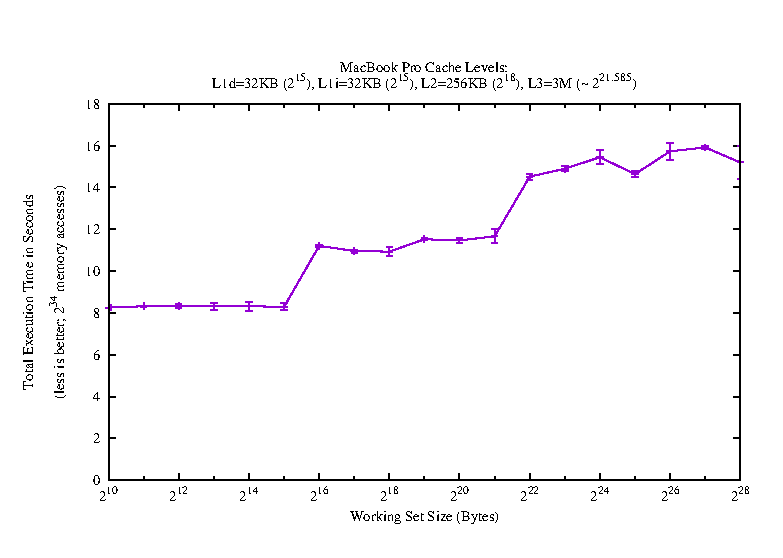
\includegraphics{appendix/plots-cache-measurements/plot-correct-ll}
\caption{Correct: Linked List, Sequential Access, and Single Loop}
\label{app:correct-ll-seqacc-sl}
\end{figure}

\begin{figure}[htbp]
\centering
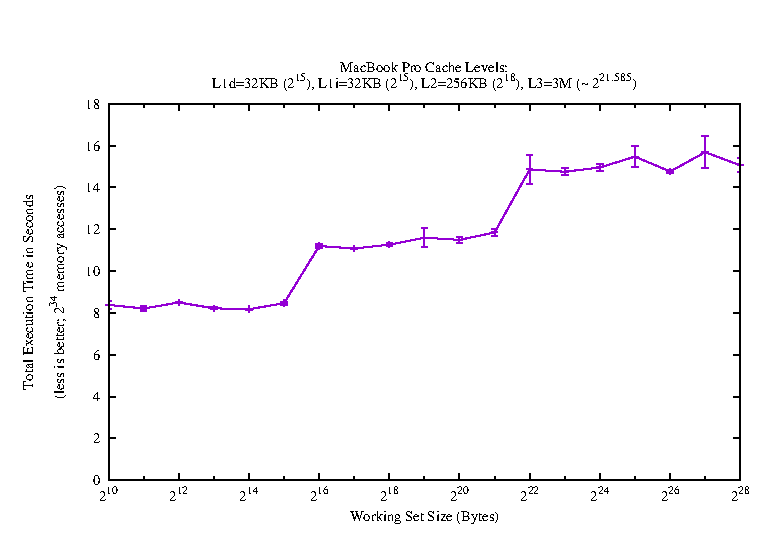
\includegraphics{appendix/plots-cache-measurements/plot-correct-array}
\caption{Correct: Array, Sequential Access, and Single Loop}
\label{app:correct-arr-seqacc-sl}
\end{figure}

\begin{figure}[htbp]
\centering
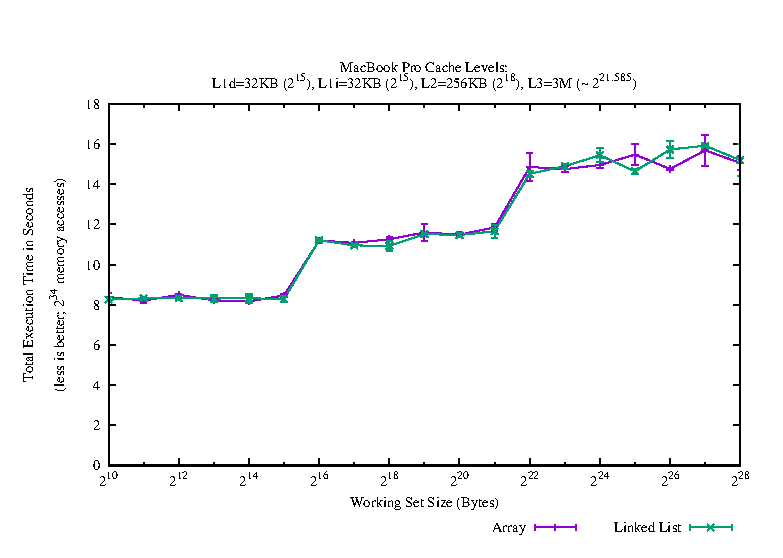
\includegraphics{appendix/plots-cache-measurements/plot-correct-array-ll}
\caption{Correct: Array, Sequential Access All, and Single Loop}
\label{app:correct-arr-seqaccall-sl}
\end{figure}

\hypertarget{big-iron9}{\subparagraph{\texorpdfstring{\texttt{big-iron9}}{big-iron9}}\label{big-iron9}}

So far all experiments are done on a MacBook pro. We re-run our approach
to solve the problem on \texttt{big-iron9} to corroborate our results.

The figure on the left shows the performance using a linked list. As
expected it illustrates nicely the cache hierarchy. We observe a
significant performance decrease at a working set size of 214 which
indicates at we now working on L2. There is another decrease around 220
which shows that L2 is not enough anymore and our data is stored in L3.
Take a look at a working set size of 224 presents the last decease of
performance, now our data is stored at the main memory.

The figure on the right shows the performance using an array. Obviously,
this approach offers better performance. This is different from the
execution on the MacBook, where performance for both approaches is quite
similar. Nevertheless, the shape of this figure presents the cache
hierarchy. We are able to observe which cache level is accessed for
which working set size. Even if the difference between L1 and L2 is very
small.

The third figure illustrates the differences of array and linked list.

\begin{figure}[htbp]
\centering
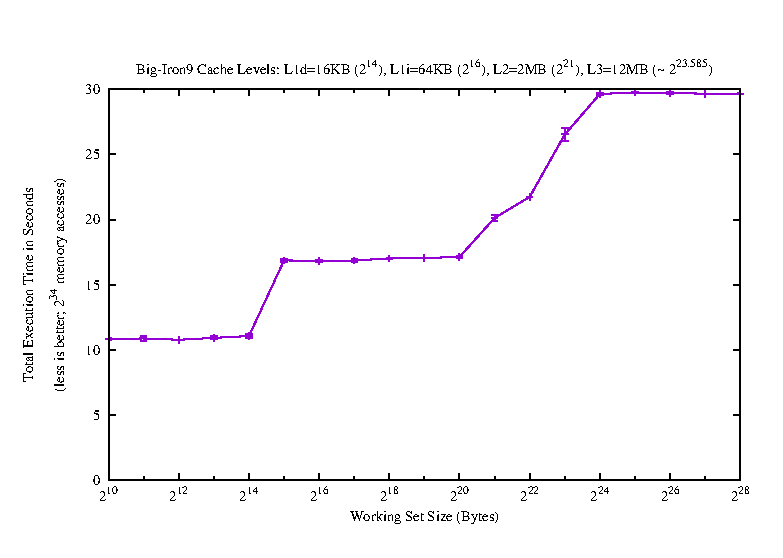
\includegraphics{appendix/plots-cache-measurements/plot-bi9-correct-ll}
\caption{Correct: Linked List, Sequential Access, and Single Loop}
\label{app:correct-ll-seqacc-sl-bi9}
\end{figure}

\begin{figure}[htbp]
\centering
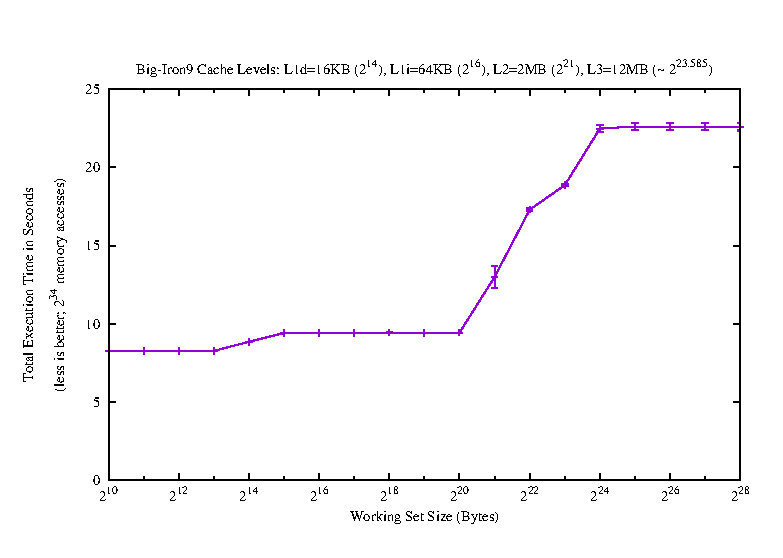
\includegraphics{appendix/plots-cache-measurements/plot-bi9-correct-array}
\caption{Correct: Array, Sequential Access, and Single Loop}
\label{app:correct-arr-seqacc-sl-bi9}
\end{figure}

\begin{figure}[htbp]
\centering
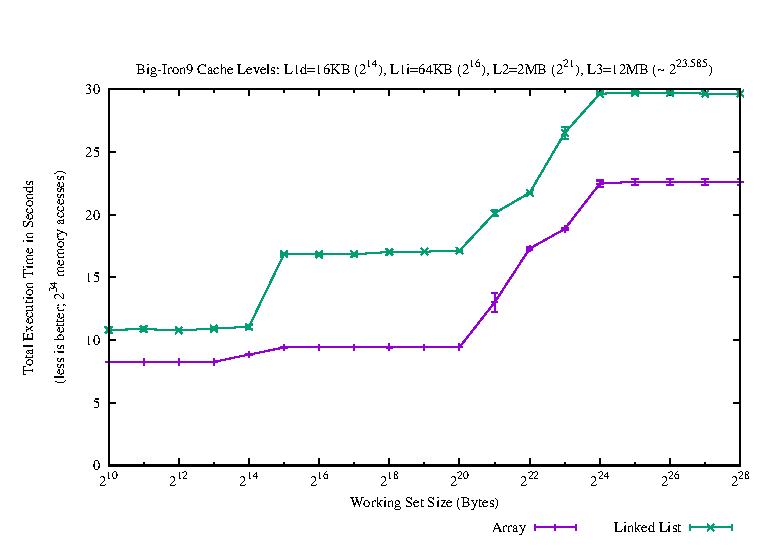
\includegraphics{appendix/plots-cache-measurements/plot-bi9-correct-array-ll}
\caption{Correct: Array, Sequential Access All, and Single Loop}
\label{app:correct-arr-seqaccall-sl-bi9}
\end{figure}

\subsection{Conclusion}\label{conclusion-5}

We started this report with experiments on different access methods of
our data structures linked list, and array, respectively. These
experiments nicely present performance differences. Furthermore, we
observe some interesting behavior for the array experiments. We define
this unexpected behavior as a problem and investigate it to find the
cause. Our investigations lead deeply into the generated assembly code.
We identified two reasons: (1) There is a special assembly command on
Intel x86 machines (\texttt{lea}) designed for array access without an
expensive memory access . (2) There are no assembly commands generated
for \texttt{C} code like \texttt{(void)cur-\textgreater{}pad{[}0{]};} if
there is no assignment. The combination of these leads to the working
set size independent performance of our array experiments. Finally, we
present a solution for this problem. Furthermore, we present experiments
which confirm the correctness of our solution.
